% Reference diagram illustrating the two DPS splitting configurations.
% This figure is not included in the PRL Letter or Supplemental Material.
% Compile in this directory with: pdflatex -interaction=nonstopmode -halt-on-error dps_sketch.tex
% Incoming partons from the two gluons are distinguished by colour.
% Momentum labels identify the loop momenta and the collinear fractions at p_T = 0.
\documentclass[tikz,border=2pt]{standalone}
\usetikzlibrary{decorations.pathmorphing,decorations.markings,arrows.meta}
\definecolor{one}{HTML}{2A78D6}
\definecolor{two}{HTML}{EB6834}
\definecolor{ink}{HTML}{0B0B0B}
\definecolor{ink2}{HTML}{52514E}
\tikzset{
  gluon/.style={decorate,draw=#1,line width=0.7pt,
                decoration={coil,aspect=0.35,segment length=4.2pt,amplitude=1.9pt}},
  quark/.style 2 args={draw=#1,line width=0.9pt,postaction={decorate},
                decoration={markings,mark=at position #2 with {\arrow[#1]{Stealth[length=5pt,width=4pt]}}}},
  boson/.style={decorate,draw=ink,line width=0.7pt,decoration={snake,amplitude=1.6pt,segment length=6pt}},
  scalar/.style={draw=ink,line width=0.8pt,dashed},
  lab/.style={font=\small,text=ink},
  frac/.style={font=\footnotesize,text=ink2},
  mom/.style={font=\small},
}
\begin{document}
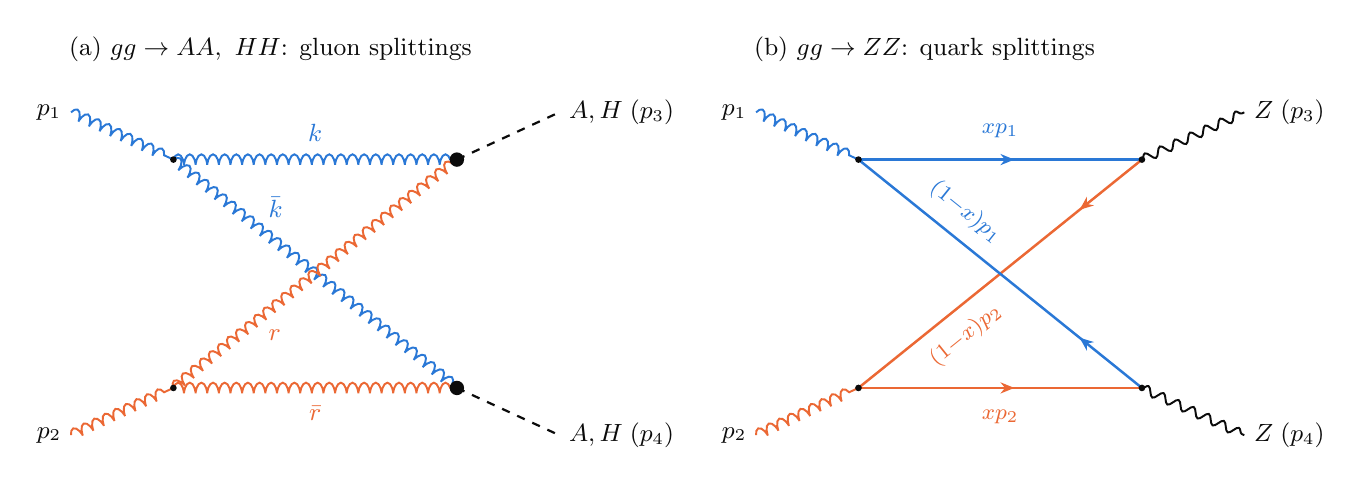
\begin{tikzpicture}[x=1cm,y=1cm]
  \def\H{2.9}                        % height of the box; its width is 3.6
  % ---------------------------------------------------------------- (a) gluon splittings
  \begin{scope}
    \coordinate (V1) at (0,\H);  \coordinate (V2) at (0,0);
    \coordinate (V3) at (3.6,\H); \coordinate (V4) at (3.6,0);
    \draw[gluon=one] (-1.3,{\H+0.6}) -- (V1);
    \draw[gluon=two] (-1.3,-0.6) -- (V2);
    \node[lab,anchor=east] at (-1.3,{\H+0.6}) {$p_1$};
    \node[lab,anchor=east] at (-1.3,-0.6) {$p_2$};
    \draw[gluon=one] (V1) -- (V3);
    \draw[gluon=one] (V1) -- (V4);
    \draw[gluon=two] (V2) -- (V3);
    \draw[gluon=two] (V2) -- (V4);
    \draw[scalar] (V3) -- (4.9,{\H+0.6});
    \draw[scalar] (V4) -- (4.9,-0.6);
    \node[lab,anchor=west] at (4.9,{\H+0.6}) {$A,H\;(p_3)$};
    \node[lab,anchor=west] at (4.9,-0.6) {$A,H\;(p_4)$};
    \fill[ink] (V3) circle (2.6pt);  \fill[ink] (V4) circle (2.6pt);
    \fill[ink] (V1) circle (1.2pt);  \fill[ink] (V2) circle (1.2pt);
    % the momenta of section 2.2: k ~ x p1, kbar ~ (1-x) p1, r ~ (1-x) p2, rbar ~ x p2
    \node[mom,text=one,above=3pt] at (1.8,\H) {$k$};
    \node[mom,text=two,below=3pt] at (1.8,0) {$\bar r$};
    \path (V1) -- (V4) node[mom,text=one,pos=0.3,anchor=south west,inner sep=3.5pt] {$\bar k$};
    \path (V2) -- (V3) node[mom,text=two,pos=0.3,anchor=north west,inner sep=3.5pt] {$r$};
    \node[lab,anchor=west] at (-1.45,{\H+1.4}) {(a) $gg\to AA,\ HH$: gluon splittings};
  \end{scope}
  % ---------------------------------------------------------------- (b) quark splittings
  \begin{scope}[xshift=8.7cm]
    \coordinate (V1) at (0,\H);  \coordinate (V2) at (0,0);
    \coordinate (V3) at (3.6,\H); \coordinate (V4) at (3.6,0);
    \draw[gluon=one] (-1.3,{\H+0.6}) -- (V1);
    \draw[gluon=two] (-1.3,-0.6) -- (V2);
    \node[lab,anchor=east] at (-1.3,{\H+0.6}) {$p_1$};
    \node[lab,anchor=east] at (-1.3,-0.6) {$p_2$};
    % one fermion loop V1 -> V3 -> V2 -> V4 -> V1; the quark leaving each gluon vertex and the
    % antiquark arriving at it are both collinear to that gluon
    \draw[quark={one}{0.55}] (V1) -- (V3);
    \draw[quark={two}{0.22}] (V3) -- (V2);
    \draw[quark={two}{0.55}] (V2) -- (V4);
    \draw[quark={one}{0.22}] (V4) -- (V1);
    \draw[boson] (V3) -- (4.9,{\H+0.6});
    \draw[boson] (V4) -- (4.9,-0.6);
    \node[lab,anchor=west] at (4.9,{\H+0.6}) {$Z\;(p_3)$};
    \node[lab,anchor=west] at (4.9,-0.6) {$Z\;(p_4)$};
    \foreach \v in {V1,V2,V3,V4} \fill[ink] (\v) circle (1.2pt);
    \node[frac,text=one,above] at (1.8,{\H+0.15}) {$xp_1$};
    \node[frac,text=two,below] at (1.8,-0.15) {$xp_2$};
    \path (V1) -- (V4) node[frac,text=one,pos=0.32,sloped,above=2pt] {$(1{-}x)p_1$};
    \path (V2) -- (V3) node[frac,text=two,pos=0.32,sloped,below=2pt] {$(1{-}x)p_2$};
    \node[lab,anchor=west] at (-1.45,{\H+1.4}) {(b) $gg\to ZZ$: quark splittings};
  \end{scope}
\end{tikzpicture}
\end{document}
